\section{Вещественные числа}
\index{R@$\mathbb R$} \index{Число!вещественное} Множество вещественных чисел обозначается $\mathbb R$.

\subsection{Аксиоматика вещественных чисел}
Аксиомы сложения:
\begin{enumerate}
	\item Коммутативность сложения: $\forall a, b \in \mathbb R \ a + b = b + a$
	\item Ассоциативность сложения: $\forall a, b, c \in \mathbb R \ a + (b + c) = (a + b) + c$
	\item Существование \textbf{нуля}: $\exists 0 \in \mathbb R \colon \forall a \in \mathbb R \ a + 0 = a$
	\item Существование \textbf{противоположного} числа: $\forall a \in \mathbb R \ \exists (-a) \in \mathbb R \colon a + (-a) = 0$
\end{enumerate}

Аксиомы умножения:
\begin{enumerate}
	\item Коммутативность умножения: $\forall a, b \in \mathbb R \ a \cdot b = b \cdot a$
	\item Ассоциативность умножения: $\forall a, b, c \in \mathbb R \ a \cdot (b \cdot c) = (a \cdot b) \cdot c$
	\item Дистрибутивность умножения относительно сложения: $\forall a, b, c \in \mathbb R \ a \cdot (b + c) = a \cdot b + a \cdot c$
	\item Существование \textbf{единицы}: $\exists 1 \in \mathbb R \colon \forall a \in \mathbb R \ a \cdot 1 = a$
	\item Существование \textbf{обратного} числа: $\forall a \in \mathbb R \setminus \{ 0 \} \ \exists \frac1a = a^{-1} \in \mathbb R \colon a \cdot a^{-1} = 1$
\end{enumerate}

Аксиомы порядка:
\begin{enumerate}
	\item Рефлексивность: $\forall a \in \mathbb R \ a \leqslant a$
	\item Антисимметричность: $\forall a, b \in \mathbb R \ a \leqslant b \lAnd b \leqslant a \Rightarrow a = b$
	\item Транзитивность: $\forall a, b, c \in \mathbb R \ a \leqslant b \lAnd b \leqslant c \Rightarrow a \leqslant c$
	\item Линейная упорядоченность: $\forall a, b \in \mathbb R \ a \leqslant b \lOr b \leqslant a$
	\item Связь сложения и порядка: $\forall a, b, c \in \mathbb R \ a \leqslant b \Rightarrow a + c \leqslant b + c$
	\item Связь умножения и порядка: $\forall a, b \in \mathbb R \ 0 \leqslant a \lAnd 0 \leqslant b \Rightarrow 0 \leqslant a \cdot b$
\end{enumerate}

Аксиома нетривиальности: $0 \neq 1$

\hypertarget{eq:continuity_axiom}{Аксиома непрерывности}: $\forall A, B \subset \mathbb R \colon
(\forall a \in A, \ b \in B \ a \leqslant b) \
\exists x \in \mathbb R \colon
a \leqslant x \leqslant b$

\subsection{Существование иррациональных чисел}
\index{I@$\mathbb I$} \index{Число!иррациональное} \textbf{Иррациональным} называется число, не являющееся рациональным.
Множество иррациональных чисел обозначается $\mathbb I$.

\begin{statement}
Существуют иррациональные числа.
\end{statement}
\begin{proofcontra}
Пусть $\exists p \in \mathbb Z, \ q \in \mathbb N \colon \left( \frac{p}q \right)^2 = 2 \lAnd \NOD(p, q) = 1$.
Тогда
\begin{equation*}
p^2 = 2q^2 \Rightarrow p^2 \mult 2 \Leftrightarrow p \mult 2
\Leftrightarrow p = 2l \lAnd l \in \mathbb Z \Rightarrow 2l^2 = q^2
\end{equation*}

Аналогичными рассуждениями получим $q \mult 2$.
$p \mult 2 \lAnd q \mult 2 \Rightarrow \NOD(p, q) \neq 1$.
Противоречие.
\end{proofcontra}

\begin{statement}
Среди вещественных чисел есть иррациональные.
\end{statement}
\begin{proof}
Пусть $X = \{ x \in \mathbb R^+ \mid x^2 < 2 \}$, $Y = \{ y \in \mathbb R^+ \mid y^2 > 2 \}$.
\begin{equation*}
\forall x \in X, \ y \in Y \ y^2 - x^2 = (y - x)(y + x) > 0 \Rightarrow y > x \Rightarrow
\exists z \in \mathbb R \colon \forall x \in X, \ y \in Y \ x \leqslant z \leqslant y
\end{equation*}

\begin{enumerate}
	\item Пусть $z^2 < 2$. $z \in X$, $z > 1{,}1$, тогда
	\begin{equation*}
	0 < 2 - z^2 < 1 \Rightarrow \frac{2 - z^2}5 < 1 \Rightarrow
	\left( \frac{2 - z^2}5 \right)^2 < \frac{2 - z^2}5
	\end{equation*}
	
	\begin{itemize}
		\item $\displaystyle z + \frac{2 - z^2}5 > z \Rightarrow z + \frac{2 - z^2}5 \notin X$
		
		\item $\displaystyle \left( z + \frac{2 - z^2}5 \right)^2 =
		z^2 + 2z\cdot\frac{2 - z^2}5 + \left( \frac{2 - z^2}5 \right)^2 <
		z^2 + \frac45 (2 - z^2) + \frac{2 - z^2}5 = 2 \Rightarrow z + \frac{2 - z^2}5 \in X$
	\end{itemize}
	Противоречие, значит, $z^2 \geqslant 2$.
	
	\item Пусть $z^2 > 2$. $z \in Y$, $z < 1{,}9$, тогда
	\begin{equation*}
	0 < z^2 - 2 < 2 \Rightarrow \frac{z^2 - 2}4 < 1 \Rightarrow
	\left( \frac{z^2 - 2}4 \right)^2 < \frac{z^2 - 2}4
	\end{equation*}
	
	\begin{itemize}
		\item $\displaystyle z - \frac{z^2 - 2}4 < z \Rightarrow z + \frac{z^2 - 2}4 \notin Y$
		
		\item $\displaystyle \left( z - \frac{z^2 - 2}4 \right)^2 =
		z^2 - z\cdot\frac{z^2 - 2}2 + \left( \frac{2 - z^2}4 \right)^2 >
		z^2 - (z^2 - 2) = 2 \Rightarrow z - \frac{z^2 - 2}4 \in Y$
	\end{itemize}
	
	Противоречие, значит, $z^2 \leqslant 2$.
\end{enumerate}

Т.\,о., $z^2 \leqslant 2 \lAnd z^2 \geqslant 2 \Leftrightarrow z^2 = 2 \Rightarrow
\exists z \in \mathbb R \colon z^2 = 2 \Rightarrow z \notin \mathbb Q$.
\end{proof}

\subsection{Геометрическое представление вещественных чисел}
Самой распространённой интерпретацией множества~$\mathbb R$ является бесконечная прямая.
\begin{figure}[H] \centering
\noindent
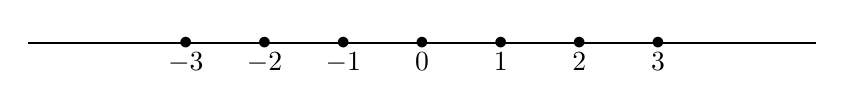
\begin{tikzpicture}
\draw (-5, 0) -- (5, 0);
\foreach \x in {-3, ..., 3}
	\draw (\x, 0) node {$\bullet$} node[below] {$\x$};
\end{tikzpicture}
\caption{Множество~$\mathbb R$ в~виде прямой}
\end{figure}

Множество~$\mathbb R$ также можно представить в~виде окружности, одна точка которой соответствует нулю, а другая~--- бесконечности.
\begin{figure}[H] \centering
\noindent
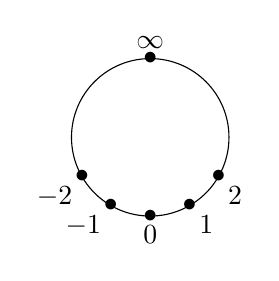
\begin{tikzpicture}
\draw (0, 0) circle (1);
\def\angle#1{#1*30-90}
\def\drawpoint#1#2#3{% {угол}{надпись}{параметры надписи}
	\draw (#1:1) node {$\bullet$} node[#3] {$#2$}
}

\foreach \x in {-2, -1}
	\drawpoint{\angle{\x}}{\x}{below left};
\drawpoint{\angle{0}}{0}{below};
\foreach \x in {1, 2}
	\drawpoint{\angle{\x}}{\x}{below right};
\drawpoint{90}{\infty}{above};
\end{tikzpicture}
\caption{Множество~$\mathbb R$ в~виде окружности}
\end{figure}

\begin{wrapfigure}{r}{0pt} %54mm
\noindent
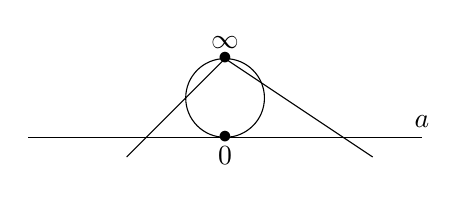
\begin{tikzpicture}[scale=0.5]
\draw (-5, 0) -- (0, 0) node {$\bullet$} node[below] {$0$} -- (5, 0) node[above] {$a$};
\draw (0, 1) circle (1);
\draw (0, 2) coordinate (I) node {$\bullet$} node[above] {$\infty$};
\draw (I) -- (3.75, -0.5)
	(I) -- (-2.5, -0.5);
\end{tikzpicture}
\end{wrapfigure}
Покажем, что эти интерпретации взаимозаменяемы.
Изобразим их так, чтобы точка, соответствующая нулю на прямой~$a$, совпадала с точкой, соответствующей нулю на окружности.
Теперь из точки, соответствующей бесконечности на окружности, проведём все возможные прямые.
Каждая из них пересекает одну точку на прямой~$a$ и одну точку на окружности и таким образом устанавливает взаимно однозначное соответствие, при этом $-\infty$ и $+\infty$ означают движение к одной и той~же точке на окружности, соответствующей бесконечности.